
\begin{frame}
  \frametitle{Object-based Over-decomposition}
  \begin{itemize} 
    \item Let the programmer decompose computation into objects
    \begin{itemize}
       \item Work units, data-units, composites
    \end{itemize}
    \item Let an intelligent runtime system assign objects to processors
    \begin{itemize}
      \item RTS can change this assignment (mapping) during execution
      \item Locality of data references is a critical attribute for performance 
      \item A parallel object can access only its own data
      \item Asynchronous method invocation for accessing other objects’ data
      \item RTS can schedule work whose dependencies have been satisfied
    \end{itemize}
\end{itemize}
\end{frame}

% \begin{frame}
%  \frametitle{Object Boundaries}
%     \begin{itemize}
%       \item Parameters to methods of objects represent data dependencies
%       \item Programmer designs objects and methods with explicit dependencies
%       \item Flow of control is then the chain of dependencies
%       \item Overlap of independent computations happens automatically as dependencies are met via message delivery
%     \end{itemize}
%  \end{frame}

%% Grainsize slides
\begin{frame}
  \frametitle{Amdahl’s Law and Grainsize}
  \begin{itemize}
    \item Original ``law'':
      \begin{itemize}
      \item If a program has $K$\% sequential section, then speedup is limited
        to $\frac{100}{K}$.
        \begin{itemize}
        \item If the rest of the program is parallelized completely
        \end{itemize}
      \end{itemize}
    \item Grainsize corollary:
      \begin{itemize}
      \item If any individual piece of work is $> K$ time units, and the
        sequential program takes $T_{seq}$, 
        \begin{itemize}
        \item Speedup is limited to $\frac{T_{seq}}{K}$
        \end{itemize}
      \end{itemize}
    \item So:
      \begin{itemize}
      \item Examine performance data via histograms to find the sizes of
        remappable work units
      \item If some are too big, change the decomposition method to make
        smaller units
      \end{itemize}
  \end{itemize}
\end{frame}

\begin{frame}
  \frametitle{Grainsize}
  \begin{itemize}
    \item (working) Definition: the amount of computation per potentially
      parallel event (task creation, enqueue/dequeue, messaging,
      locking, etc.)
  \end{itemize}
  \begin{center} 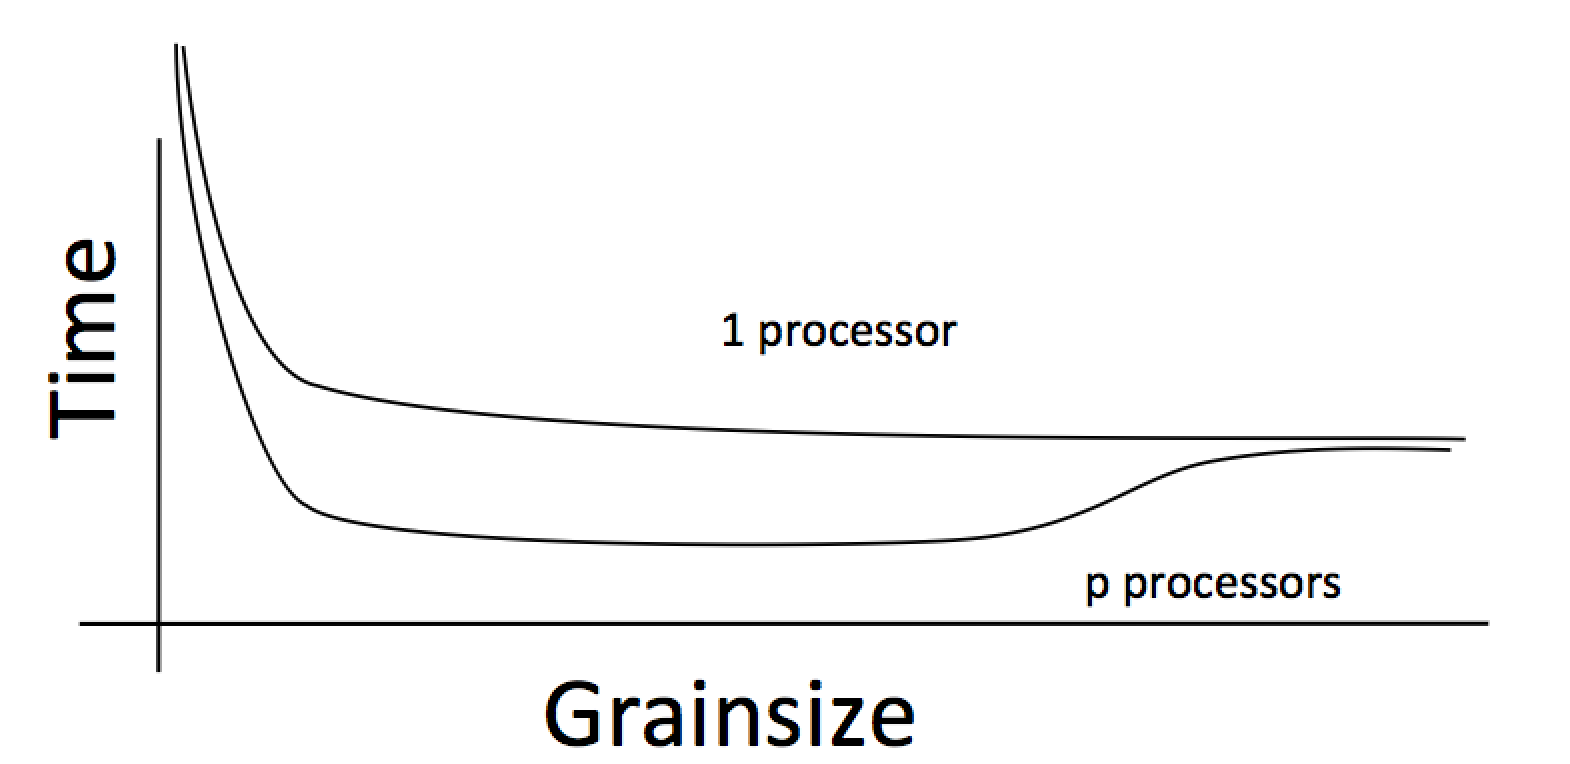
\includegraphics[width=0.7\textwidth]{figures/grain1.png} \end{center}
\end{frame}

\begin{frame}
  \frametitle{Grainsize and Overhead}
  \begin{itemize}
    \item What is the ideal grainsize?
    \item Should it depend on the number of processors?
    
  \end{itemize}
  \begin{center}
    $T_1 = T \left( 1 + \frac{v}{g} \right)$\\
    $T_p = max \left\{ g, \frac{T_1}{p} \right\}$\\
    $T_p = max \left\{ g, \frac{T\left( 1+ \frac{v}{g} \right)}{p} \right\}$\\
    $v$: overhead per message,\\
    $T_p$: $p$ processor completion time\\
    $g$: grainsize (computation per message)
  \end{center}
\end{frame}

\begin{frame}
  \frametitle{Grainsize and Scalability}
  \begin{center} 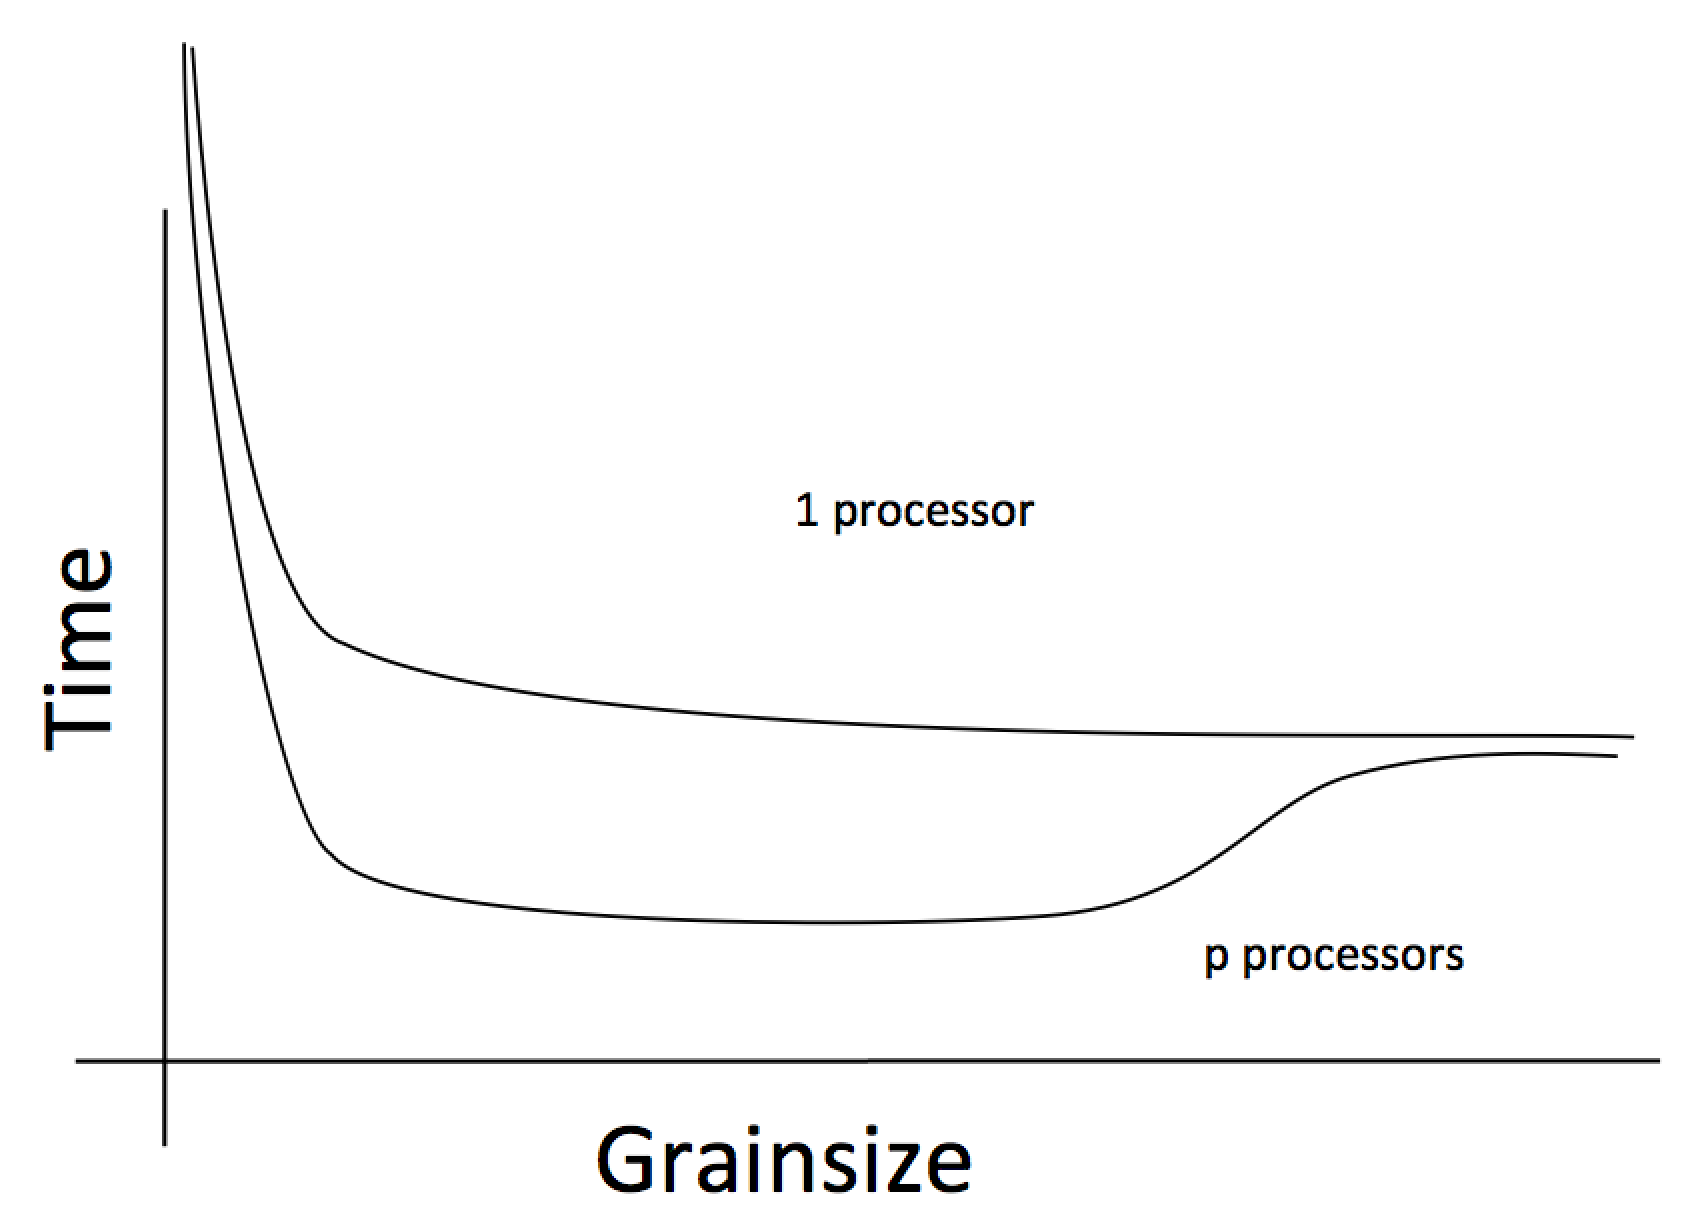
\includegraphics[width=0.7\textwidth]{figures/grain2.png} \end{center}
\end{frame}

\begin{frame}
  \frametitle{Rules of thumb for grainsize}
  \begin{itemize}
    \item Make it as small as possible, as long as it amortizes the overhead
    \item More specifically, ensure:
      \begin{itemize}
      \item \textit{Average} grainsize is greater than $kv$ (say $10v$)
      \item No single grain should be allowed to be too large 
        \begin{itemize}
          \item Must be smaller than $\frac{T}{p}$, but actually we can express
            it as:
          \item Must be smaller than $kmv$ (say $100v$)
        \end{itemize}
      \end{itemize}
    \item Important corollary:
      \begin{itemize}
      \item You can be at close to optimal grainsize without having to think
        about $p$, the number of processors
      \end{itemize}
    \item $kv < g < mkv$ ($10v < g < 100v$)
  \end{itemize}
\end{frame}

% \begin{frame}
%   \frametitle{How to determine/ensure grainsize}
%   \begin{itemize}
%     \item Compiler techniques can help, but only in some cases
%       \begin{itemize}
%         \item Note that they don't need precise determination of grainsize,
%           just one that will satisfy a broad inequality
%       \end{itemize}
%   \end{itemize}
% \end{frame}

% \begin{frame}[fragile]
%   \frametitle{Performance of Fibonacci Example}
%   \begin{itemize}
%   \item How much work/computation does each object do in this example?
%   \item What are some of the overheads of this approach?
%   \item Is there way we can reduce/amortize the overhead?
%   \end{itemize}
% \end{frame}

\begin{frame}[fragile]
  \frametitle{Grain size for Fibonacci Example}
  \begin{itemize}
  \item Set a sequential threshold in the computational tree
    \begin{itemize}
    \item Past this threshold (i.e. when $n < threshold$), instead of
      constructing two new chares, compute the fibonacci sequentially
    \end{itemize}
  \end{itemize}
  \begin{center} 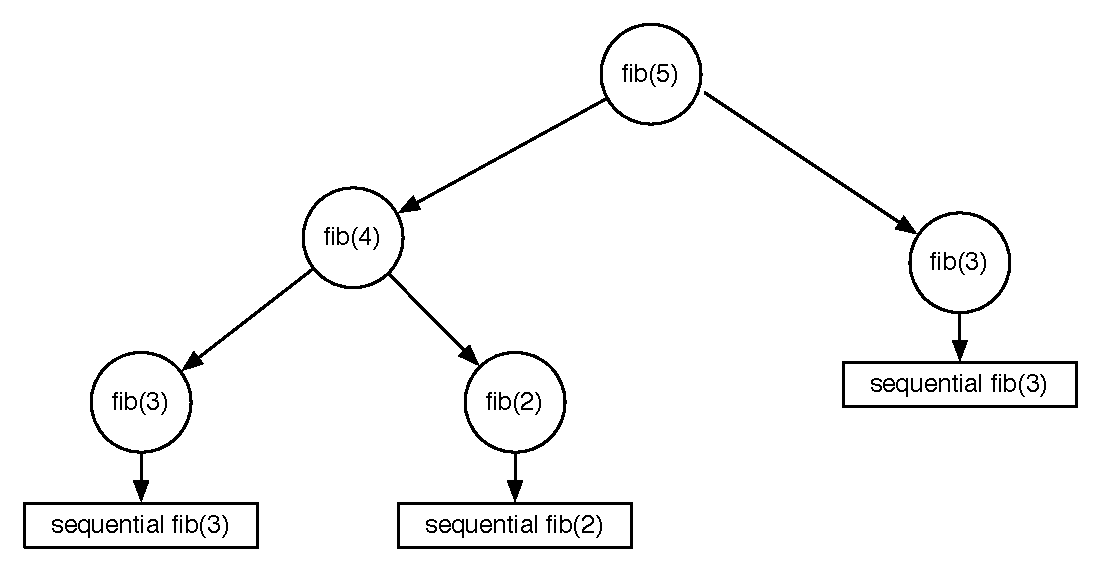
\includegraphics[width=0.7\textwidth]{figures/tree-threshold.pdf} \end{center}
  \begin{itemize}
    \item $fib(5), fib(4)$ are fine grains, $fib(3), fib(2)$ are coarser grains
    \item The coarser grains now amortize the cost of the fine-grained execution
  \end{itemize}
\end{frame}

% \begin{frame}[fragile]
%   \frametitle{Fibonacci w/Threshold Example}
%   \lstinputlisting[basicstyle=\tiny]{code/fib2.C}
% \end{frame}
